\section{Example}
We shall now look at an example, with explanations and code.
\begin{quote}
    \textbf{Objective :} To find the solubility of a molecule in a solvent. 
\end{quote}
We will be using the MoleculeNet \cite{noauthor_torch_geometricdatasets_nodate} dataset's ESOL dataset. 
\begin{quote}
    "ESOL is a small dataset consisting of water solubility data for 1128 compounds. The dataset has been used to train models that estimate solubility directly from chemical structures (as encoded in SMILES strings)."
\end{quote}
\begin{figure}
     \centering
     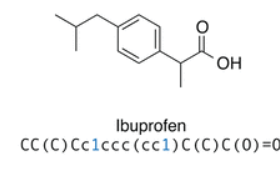
\includegraphics[width= 0.4\textwidth]{pics/smile.png}
     \caption{Smile String of Ibuprofen}
     \label{Smile}
     %add_ref
\end{figure}
Each molecule is represented as a graph, with the nodes representing the atoms. Each node (atom) has a feature vector associated with it. Since the molecule itself is represented as a graph and we would like to find the solubility of the molecule, we are naturally going to make graph level predictions. The GNN architectures vary for different levels of predictions (see section \ref{section_classification}). 

\begin{quote}
    Since this is a graph level task a Pooling layer combines the node representations of the graph into one representation so that every graph is converted to a vector embedding.
\end{quote}

3 simple GCN layers were applied followed by global Max and global Mean pooling of the graph concatenated. 

See Appendix in page \pageref{appsrccode} for some example code.